\documentclass[conference]{IEEEtran}
% \usepackage{jfrExamplee}
\usepackage{graphicx}
% \usepackage{apalike}
\usepackage{setspace}
\usepackage{cite}
\usepackage{tabularx,booktabs}

\newcolumntype{C}{>{\centering\arraybackslash}X} 
\setlength{\extrarowheight}{1pt} % for a bit more open "look"

%% Uncomment line below for double spacing
%\doublespacing

\begin{document}

\title{Visualizing Model Memorization using Explainable AI (GradCAM) as Debug Tool*\\
{\footnotesize \textsuperscript{*}Note: title is under construction}
\author{
Rawan Mahdi\thanks{ Work done during internship at the McMaster Center for Software Certification (McSCert) under the supervision of Dr. Richard Paige} \\
Department of Computing and Software\\
McMaster University\\
Hamilton, ON  \\
\texttt{mahdir3@mcmaster.ca} \\
}
}

\maketitle
% OLD TITLE AND AUTHORS TEMPLATE
% \title{Visualizing Overfitting in Convolutional Models using GradCAM}

% \And
% Coauthor \\
% Affiliation \\
% Address \\
% \texttt{email} \\
% \AND
% Coauthor \\
% Affiliation \\
% Address \\
% \texttt{email} \\
% \And
% Coauthor \\
% Affiliation \\
% Address \\
% \texttt{email} \\
% \And
% Coauthor \\
% Affiliation \\
% Address \\
% \texttt{email} \\
% }

% The \author macro works with any number of authors. There are two commands
% used to separate the names and addresses of multiple authors: \And and \AND.
%
% Using \And between authors leaves it to \LaTeX{} to determine where to break
% the lines. Using \AND forces a linebreak at that point. So, if \LaTeX{}
% puts 3 of 4 authors names on the first line, and the last on the second
% line, try using \AND instead of \And before the third author name.

%------------------------ ABSTRACT ------------------------
% \maketitle
% \begin{abstract}
% The abstract should be one paragraph. It should summarize the
% problem, approach, and significance of the results.


% \end{abstract}
%------------------------ INTRODUCTION ------------------------
\section{Introduction}

The rise in popularity of explainable AI (XAI) over the past decade has yielded a slew of XAI use cases for end-users, practitioners, and ML developers. For developers in particular, plenty of articles \cite{defuse}, \cite{revisitingsanity}, \cite{peeking} have made promising claims that XAI has the potential to provide new means of model debugging and evaluation. That being said, few studies formally propose methods to use XAI as a debugging tool, the majority applying explainability methods to well functioning models. 


While efforts are being made to develop techniques for model interpretability and explainability, the trade-off between model complexity and interpretability remains a challenge. Highly parameterized models, such as neural networks, are considered ``black boxes'' because their learning is based on heuristics \cite{heuristics}. As a result, understanding how they reach their conclusions is not straightforward or intuitive.
Relying on traditional metrics alone may be misleading in assessing such heuristic-based machine learning models. For instance, it has been shown that model performance on held out testing data could lead to overestimation of the model's generalization capability. Consequently, it exposes the model to the risk of poor performance after deployment \cite{imagenet}, \cite{beyond}, \cite{defuse}. 
In saftey-critical domains, such as healthcare and clinical decision support, this risk is magnified by it's capacity to impact patient health \cite{CDS}. 

Another area of concern stemming from a lack of interpretability is understanding what patterns have been learnt by black box models. 
- overfitting
- memorization 
- preformance and privacy issues

(OTHER BLURBS THAT WERE REMOVED)
The difficulty for practitioners of understanding what patterns have been learnt by a black box models presents challenges in evaluating such models in the context of healthcare \cite{medicalsaftey}. 

In the field of machine learning, there is a persistent need for new evaluation methods to be developed as model complexities and architectures continue to change. A number of studies have shown that traditional machine learning metrics may be misleading.


Information leakage due to the data memorization behaviour of models poses privacy concerns \cite{membershipinference}.

Of particular concern are safety critical applications of decision support systems, such as medical diagnosis and judicial decisions. (problem of memorization in safety critical domains)
Verification and validation of health safety critical models   
% diagnosis of model behavuiour
% Hook
%  - problem of generalization in machine learning and number of causes of overfitting
%  - black box models and explainability for debugging and identifying issues in the model
%  - applications in healthcare

% mitigation of distrust with medical diagnostic models

% industry standard explanations for medical images - post-hoc salinecy methods \cite{systemtatic} - gradCAM is fast 
% GDRP

% CDSS - clinical decision support system [u]

% mobile healthcare, remote diagnosis, etc
\subsection{Our Contributions}
In this study, we propose a means of model evaluation, using GradCAM to visually identify non-generalized models. We hypothesized that models that memorize during training, i.e. non-generalized models, will have visibly different feature attribution behaviour, evident through their class activation maps. If that were the case, we would be able to diagnose a model’s memorization behaviour based on it’s class activation map, giving developers greater insight into their model's decision making process. To test this hypothesis, we trained 7 models, each varying in it's architecture or training data, and hence reflect different training and testing performance. We then observed the GradCAM outputs for each model, looking for visual patterns that reflect the internal behaviour of the model. Our findings were that gradient-based activation maps differ in their visual characteristics based on the model's generalization, and reflect whether or not the model has learnt patterns from the data rather than memorizing it. 
% \begin{figure} [h]
%     \centering
%     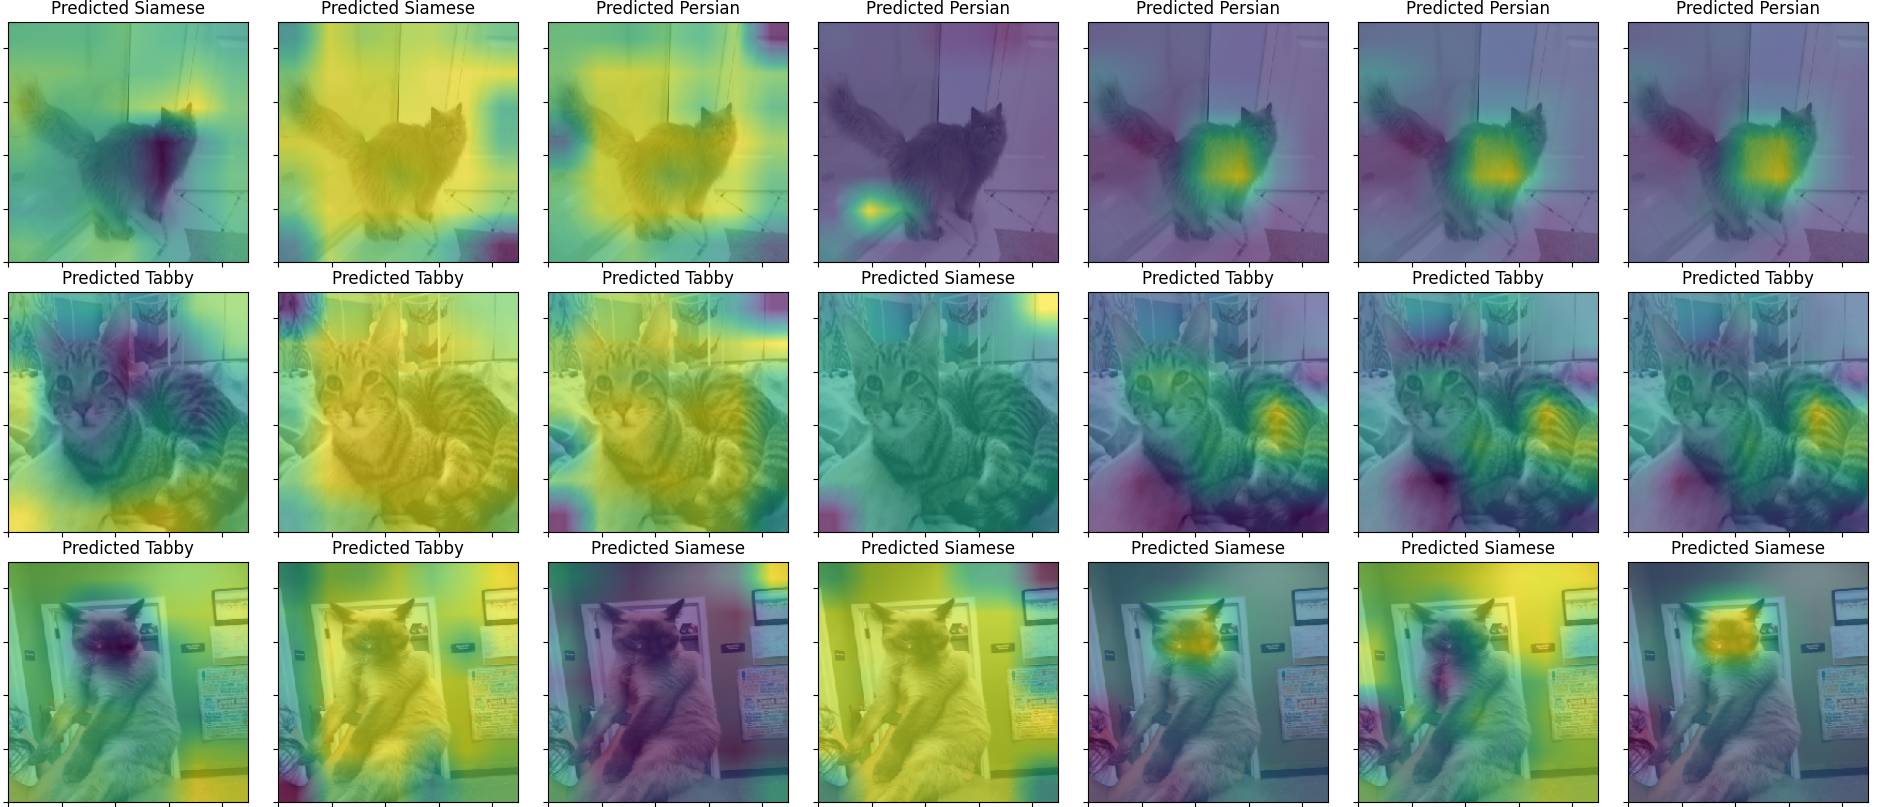
\includegraphics[height=.9in]{imgs/cat_grids/intro_pic.png}
%     \caption{three sample}
%     \label{fig:introheatmaps}
% \end{figure}
\subsection{Structure of Paper}
The paper is structured as follows:
\begin{itemize}
    \item In section 2, we give an overview of previous work that guided and inspired our contributions;
    \item In section 3, we cover our application of GradCAM on a variety of models, each differing in it's architecture, hyperparameters, or training data;
    \item In section 4, we discuss our observation based empirical evaluations of the GradCAM outputs and how they can be used to identify overfitted models;
    \item In section 5 we conclude with our findings and potential limitations in our methodology, as well as opportunities for future works to improve and build on our proposal. 
\end{itemize}
% (MENTION SOMEWHERE THAT WE USE 'overfitted' and 'non-generalized' INTERCHANGEABLY)
% (MENTION THAT WE REFER TO CROSS VALIDATION AS TRAIN-TEST Performance difference)

%------------------------ BACKGROUND ------------------------

\section{Background and Related Work}
\label{gen_inst}
 \subsection{Non-traditional Metrics}
 % \subsection{Machines that Memorize}
One of the many motivating factors behind this study is the exploration of a new metric to evaluate the behaviour of black box models. Pasa et al. show that greater performance changes are visible in saliency maps than in traditional metrics like accuracy and AUC \cite{fastchest}, implying that for image classification models, saliency maps can provide more information about the model's generalization and learnt visual patterns. Selvaraju et al. used layer-wise aggregated feature maps to spot artifacts, i.e. detected features, in a CNN's layers, opening the opportunity to debug the model's architecture in ways that traditional metrics don't provide.  \cite{debugcnn}.

\subsection{Memorization and Generalization?}
\cite{tailabouttail}

\subsection{XAI for Generalizability}
A variety of previous studies have assessed explainability of models that overfit to confounding features in the training data, such as annotations on medical scans \cite{confounding}. Such overfitting can be identified through the use of saliency maps like GradCAM, where the developer observes the highlighted parts of the image to assess for confounding. Viviano et al. applied a regularization technique that uses attribution maps drawn by domain experts, thus training the network to ignore confounding features and learn features relevant to the image labels. They observed a weak correlation between the expert-like attribution maps and model generalization, making the argument that activation maps may not be a sufficient means of observing model generalization \cite{redherring}, however their study only focused on model's learning to associate spuriously-correlated features with the image labels rather than model memorization.

What distinguishes our study from those mentioned is that we look at weak generalization from the standpoint of the model's data memorization rather than it's learning of confounding variables, hence addressing the more general problem of overfitting caused by the inherent memorization behaviour of deep learning models \cite{labelrecorder}. To the best of our knowledge, no previous work has explored how visual model explanations vary with the models performance, reflective of the model’s architecture and regularization techniques, specifically, when the model fails to generalize due to memorization of the training dataset.

%------------------------ METHODS ---------------------
\section{Methods}
\label{methods}
\subsection{Base Model - VGG16}
\begin{figure} [h]
    \centering
    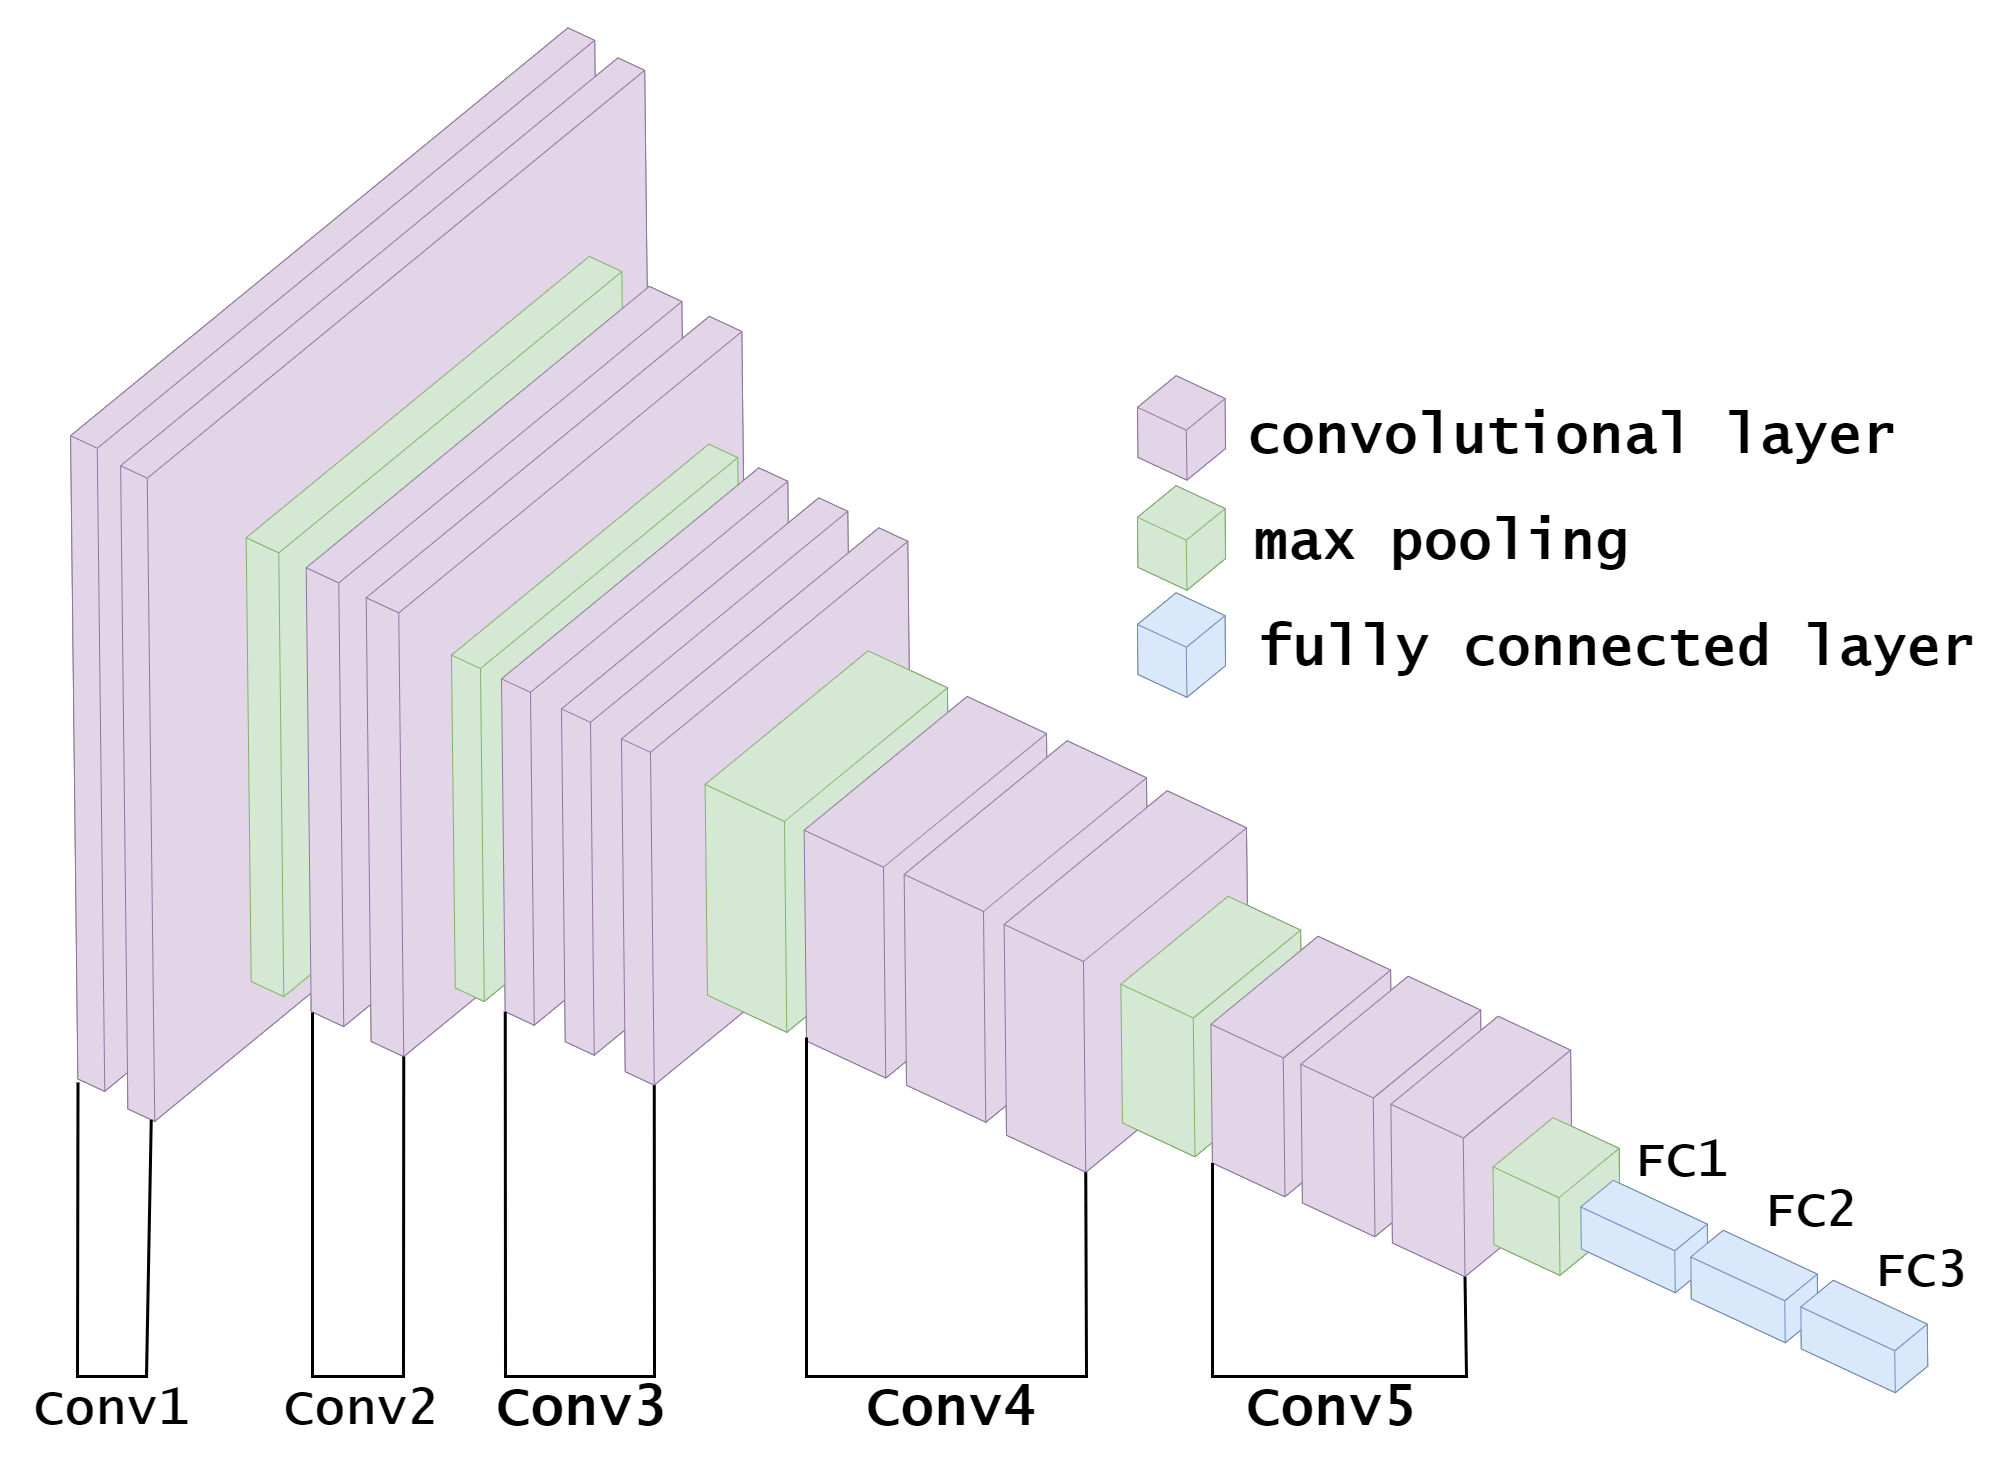
\includegraphics[height=2.5in]{imgs/VGG16architecture.png}
    \caption{VGG-16 Architecture: Models had either only their fully connected layers trained, or had both their fully connected and conv5 layers trained. Their remaining layers were transfered from the original VGG-16 model \cite{vgg16}}
    \label{fig:vgg16}
\end{figure}
Hu et al. showed that there is a positive correlation between model complexity and overfitting during training \cite{complexity}, \cite{modelcomplexity}. Since we aim to observe the behaviour of overfitted models, we chose a base model with a relatively high complexity, that being the widely recognized VGG-16 architecture \cite{vgg16}. Our goal in choosing a highly parameterized model is to have a greater representational capacity, hence aggravating the memorization of properties of the training data \cite{overandunder}, \cite{labelrecorder}, \cite{interpvscomp}. A number of studies show that, especially during transfer learning on small datasets, VGG-16 tends to overfit within a few epochs of training \cite{vgg16overfit}, \cite{vgg16overfit2}. This supports our choice in our base model, giving us the confidence that it can simulate the overfitting behaviour we want to observe in our experiments. We trained a number of models each varying in one or a combination of the following: the data it was trained on, it's hyperparameters (batch size and dropout), and the number of top layers trained. 
\begin{table*}
\caption{Model Properties and Associated Performance}
\label{models-table}
\begin{tabularx}{\textwidth}{@{} l *{10}{C} c @{}}
\toprule
model ID  
& labels & batch size & dropout & layers trained  &  training accuracy & testing accuracy  \\ 
\midrule
1   &   randomize      & 64          & 0.40   & FC1, FC2, FC3  & 0.93   & 0.32  \\ 
2 &  randomize        & 64        & 0.40    & conv5, FC1, FC2, FC3   & 0.98    & 0.30  \\ 
3       & original    & 64       & 0.00  & conv5, FC1, FC2, FC3  & 1.00   & 0.52  \\ 
4        & original       & 64          & 0.40   & conv5, FC1, FC2, FC3 & 0.82  & 0.52  \\ 
5       & original       & 256         & 0.75   &  FC1, FC2, FC3  & 0.88  & 0.86   \\ 
\addlinespace
6        & original & 256         & 0.00   &  FC1, FC2, FC3 & 1.00   & 0.85  \\ 
7       & original  &  64         & 0.40   &  FC1, FC2, FC3  & 0.98  & 0.80  \\ 
\bottomrule
\end{tabularx}
\end{table*}

% The problem of whether or not our base model will overfit to a specific dataset is undecidable \cite{overandunder} and difficult to approximate, so we chose to run a set of trials to see if we can overfit VGG16 to our dataset based on traditional metrics (train vs test accuracy and loss).  

We applied transfer learning to finetune and overfit the base model to our dataset and associated classification task. The method of transfer learning and fine-tuning involves transferring weights from the base model to the fine-tuned model up to a given layer, and retraining the weights beyond that layer to fit to the given task. Figure \ref{fig:vgg16} shows the overall VGG-16 block architecture, where five blocks of convolutional layers are followed by a neural network of three dense fully connected layers. It was observed that the most effective method of overfitting the models, i.e. getting large train-test accuracy differences, was training a greater number of top layers. Our models fall into two weight training categories: transferred weights up to the fifth convolutional block (conv5) and retrained three dense layers (FC1, FC2, FC3), or transferred weights up to conv4 and train both the conv5 block and the three dense layers. We consistently observed that the models in which the conv5 block was trained depicted greater overfitting. 
% in traditional metrics (training and testing accuracy and loss). 

\subsection{Dataset}
% - open data
% - randomized labels 
% - small size 
Our original dataset was composed of images from 3 classes of cat breeds; Tabby cats, Persian cats, and Siamese cats. All three classes were within the 1000 class ImageNet dataset that VGG-16 was trained on, however our images were sourced from open data. We maintained a relatively small data set size with the intent that this would lead to greater overfitting. As such, we split the data into 400 training samples and 100 testing samples per class. 

The testing and training datasets were independently sampled from the original distribution, via random shuffling, therefore we assume there to be no distribution gaps or confounding shifts between the two datasets \cite{invariant}. Our objective is to observe overfitting that is caused by data memorization rather than learning confounding associated with features in the images, therefore we consider our dataset to be fitting for our objective. 

As mentioned, one of the variants between our base models was the data they were trained on. We employed a popular non-parametric randomization test, closely following the variant of the test presented in \cite{generalize}, where models are trained on noise data in the form of randomized labels. 
Zhang et al. showed that models, given their architecture's effective capacity, fitted to randomized labels tend to memorize their training data, evident by their high training accuracy and the fact that there exists no correlation between the sample and it's randomly assigned label. As part of our methodology, we reproduce Zhang et al's findings through training models on random and non-random labels with the hopes of cross validating their GradCAM outputs with that of models overfitted to the original dataset. In other words, we adopt these models to act as a baseline of non-generalization to show that models overfitted to the original dataset yield similar characteristics/attribution behaviour in their heat maps. 
% our base-model, VGG-16, has the effective capacity to memorize it's training samples.

\subsection{Finetuning and Hyperparameters}
Another way we varied the level of generalization between the models in our experiment was through hyperparameters known to play a role in generalization, including dropout \cite{dropout} and batch size \cite{batchsize}. In general, increasing the dropout rate and decreasing the training batch size of our models led to greater generalization, as observed by the difference in training and testing performance in table \ref{models-table}.

\subsection{Generalization}
% In our experiment, these five models represent various levels of generalization. 
Table \ref{models-table} displays each model's associated training and testing performance, and the specific training variables of each model may be observed in table \ref{models-params}. Overfitting is traditionally identified in deep learning models via cross-validation, i.e. when training accuracy is considerably higher than testing performance \cite{theory}. Deciding exactly how much of a difference between training and testing error classifies as overfitting is generally task specific. For the sake of differentiating between the sample models we created, we will define overfitted models to be those with a difference $\geq$0.20. Therefore in this experiment, we classify models with a train-test performance difference $\leq$0.20 (models 5-7 in table \ref{models-table}) as sufficiently generalized, and have learnt some patterns relevant to the labels of the training data. 


% 

\subsection{GradCAM explanations}

% GradCAM mechanism of action + images. cite proposal. 
GradCAM heatmaps are computed through the gradient of the output neuron, i.e. the predicted class, with respect to the output of the feature map of the specified convolutional layer, that typically being the final convolutional layer \cite{gradcam}. A variety of saliency map based explainability methods have been developed, however we chose GradCAM due to it's sensitivity to model parameters and the model's pattern recognition behaviour. It has also faced notably less scrutiny than other saliency map based explanation models \cite{sanity}. We operate under the assumption that our GradCAM implementation (available here) is complete in it’s representation of the model’s decision behaviour. GradCAM has faced less scrutiny than other explaianbility methods, however some will be further considered in section \ref{discussion}. \\

% \begin{figure} [h]
%     \centering
%     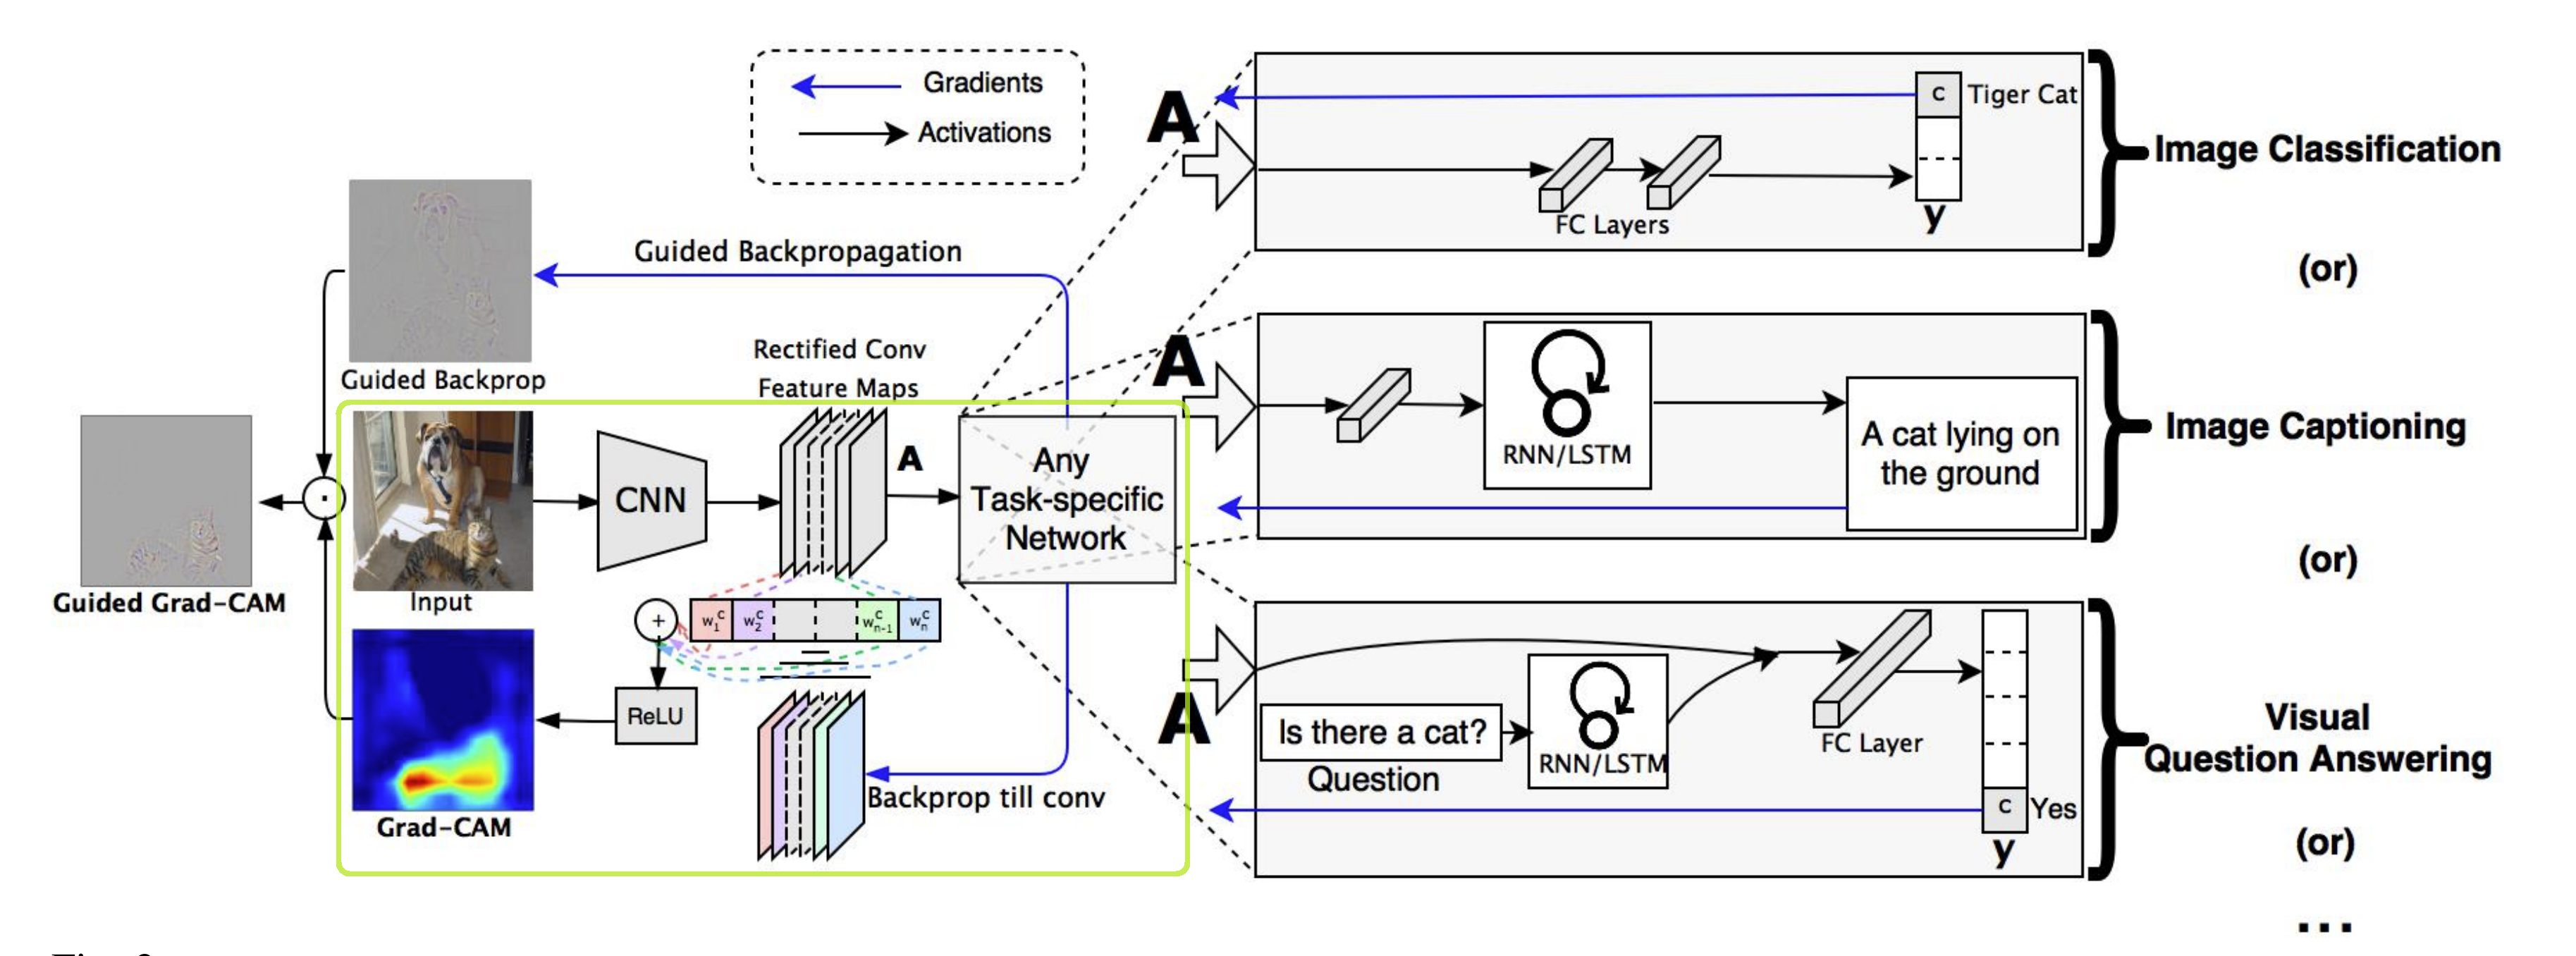
\includegraphics[height=1.3in]{GradCAM.png}
%     \caption{Overview of GradCAM, mechanisms within the green box represent those that are relevant to our system. Image reproduced from Selvaraju et al. \cite{gradcam}.}
%     \label{fig:gradcam}
% \end{figure}
Applying our implementation of GradCAM, openly available at (repo link), we obtained attribution maps for each model corresponding to randomly selected images from the training dataset.
To evaluate the output maps, we performed an informal qualitative assessment, focusing on the regions of the image that are highlighted as the brightest, most important parts of the image in regards to the classification. We judge the outputs as follows: if the brightest regions are centered around the heads and bodies of the cats in the images, we deem the model as having learnt some patterns or features of the cat breed. On the other hand, if the brightest regions of the images are not focused on the cats, or are too broad, containing too much of the background of the images, then we deem the model to have overfitted. It's important to point out that we impose a bit of intuition in our method of validating our observations. Given our classification task, identifying cat breeds, doesn't require in depth domain knowledge at our scale, we deemed our own judgement of the attribution maps to be sufficient. Imposing intuition into our method is a part of the appeal towards making the developer's model evaluation more instinctual than traditional metrics, however possible implications will be discussed in section \ref{discussion}. 

\begin{figure} [h]
    \centering
    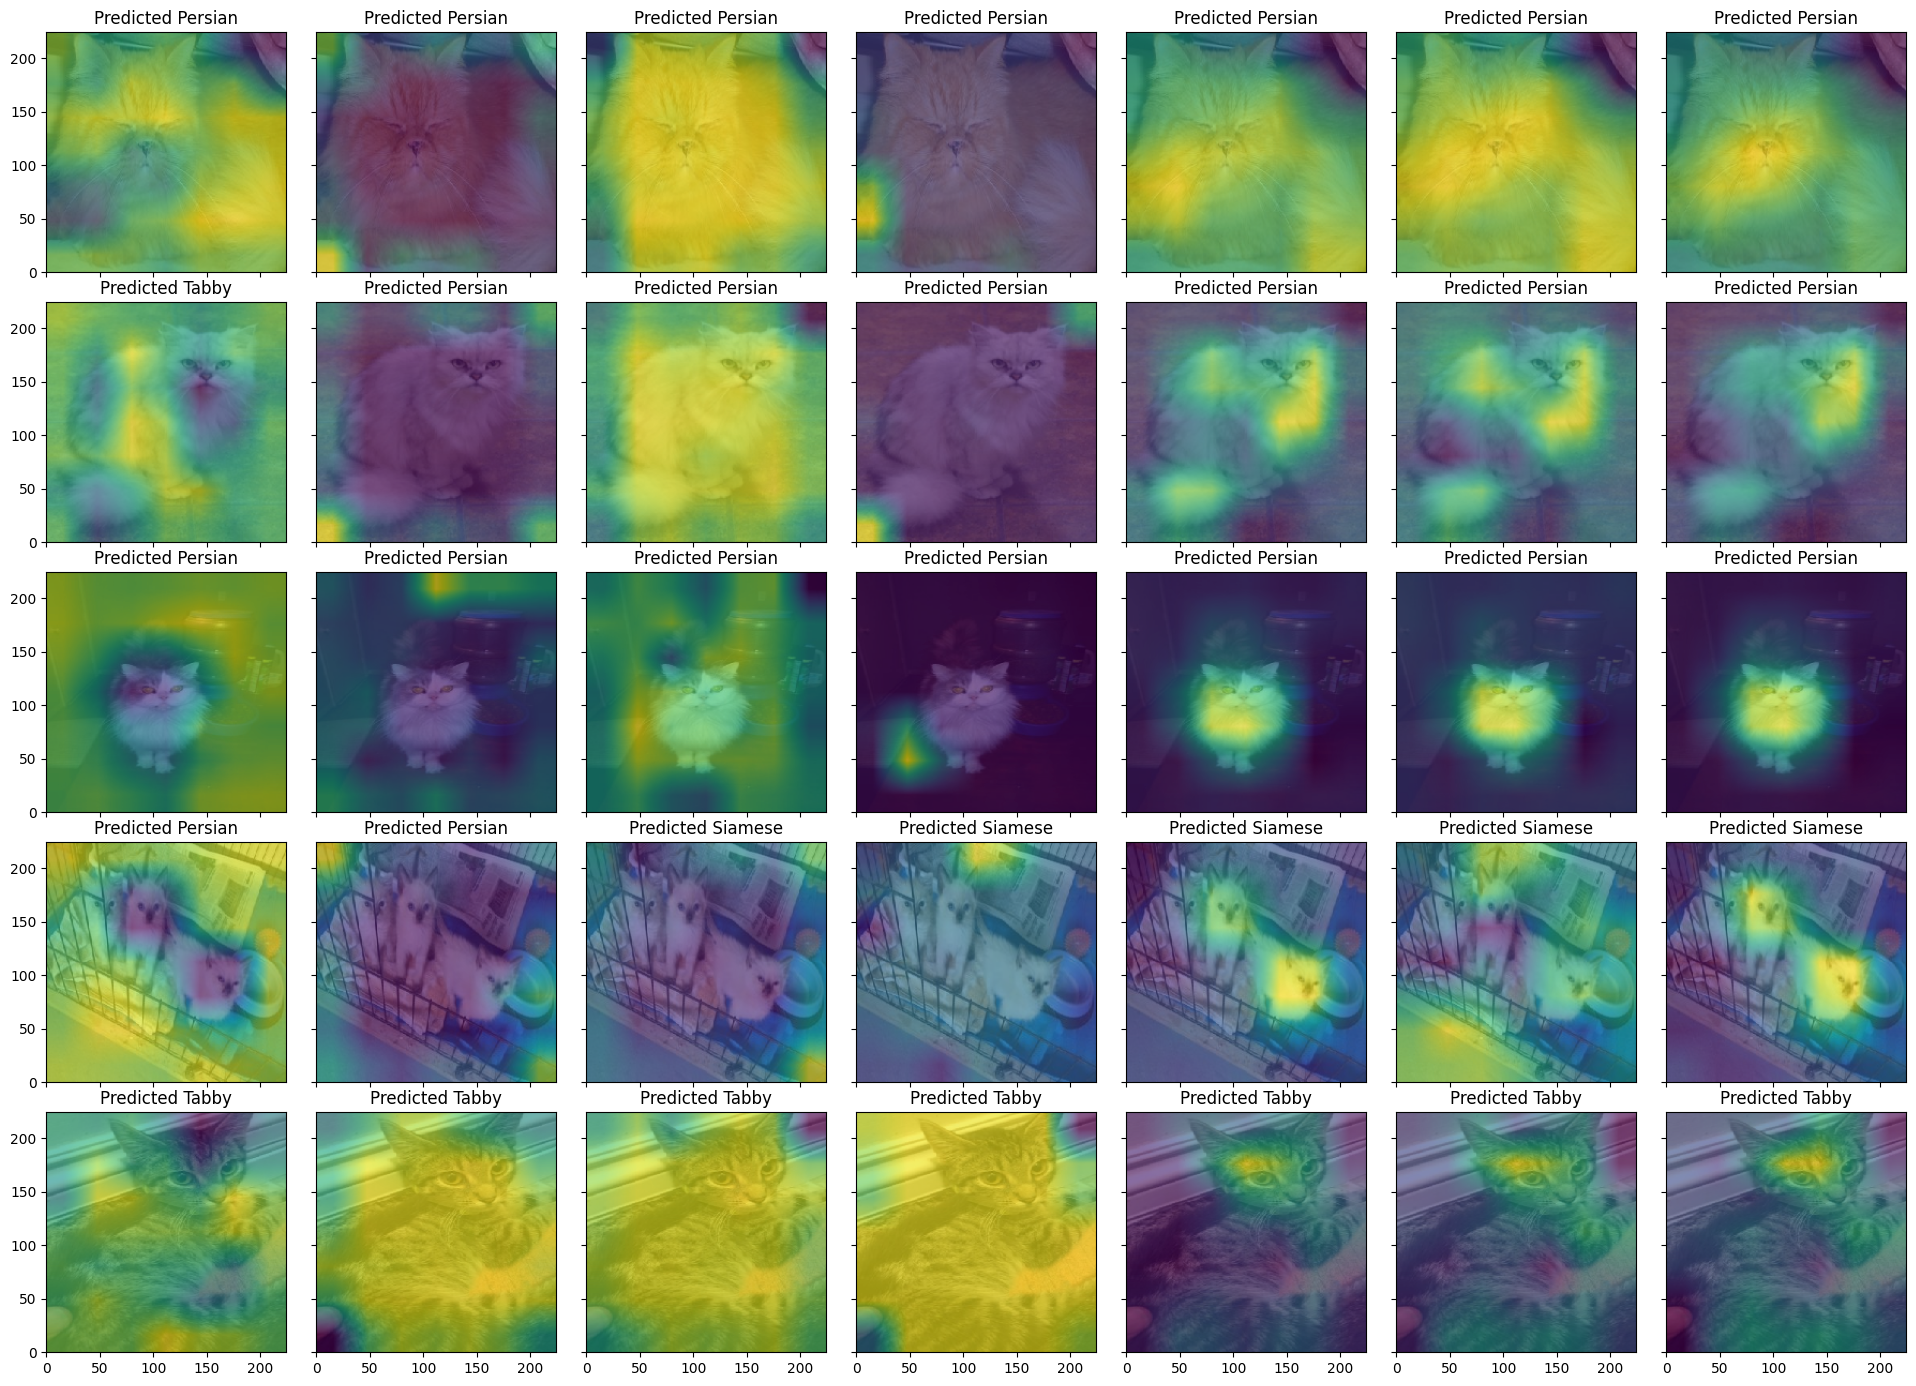
\includegraphics[height=2.5in]{imgs/cat_grids/1.png}
    \caption{GradCAM heat maps for each model across 6 images randomly selected from the testing dataset}
    \label{fig:1}
\end{figure}

% - talk about 1-4 vs 5-7
%  -- visible that models 5-7 produce similar heatmaps, with greater focus on the regions of the image that contain le chat

%------------------------ RESULTS ------------------------
\section{Observations}
Through our experiments, we were able to make the observations summarized below: 
\begin{itemize}
  \item attribution maps of well generalized models are similar to each other, but dissimilar to maps of overfitted models 
  \item overfitted models produce seemingly random or non-intuitive attribution maps, focusing on broad regions or non-distinct/irrelevant parts of the background 
\end{itemize}
% Through our approach, we were able to show that the saliency maps of models fitted to noise were notably similar to the maps of models overfitted to regular data. 
This can be observed in Figure \ref{fig:1}, where the first two columns are outputs of the models trained on noise, and the remaining columns are models trained on regular data but vary in their performance. We can see that, in general, models 5-7 highlight regions of the image that contain key features of the cats, either it's face, it's body, or both. In contrast, we see that models 1-4 highlight broad regions of the image which may contain parts of the cats and the backgrounds, or don't contain any parts of the cats. Recall that models 1-4 were identified in section \ref{methods} as non-generalized since their test train accuracy difference was greater than 0.20. Given these observations, we were able to demonstrate that overfitting is visible through GradCAM's saliency map based explanations. 

It's difficult to come to a certain and confident conclusion on the basis of our general observations, however we generated many more grids, a handful of which are available in the appendix (section \ref{appendix}), to increase confidence in the results. 
Other noteworthy findings are that in some sample images,  model 6 depicted similar attribution behaviour as models 1-4, where the background is brightest. We believe this is due to model 6 overfitting, since it's closest to our overfitting range, having test train accuracy difference of 0.15. 

There are other outliers to our observations listed above, however given that the majority of the samples fall within our observations of the overfitting behaviours, we believe they can be confidently attributed to small amounts of overfitting in models 5-7 due to the small dataset of 400 samples per class.

(strange opposite behaviour of map 1 and the generalized maps)
%------------------------ DISCUSSION ------------------------
\section{Conclusion, Limitations, and Future Works}
\label{discussion}
\subsection{GradCAM for ML Saftey?}
In this study, we observed that it is possible to identify an overfitted model from it's GradCAM explanation alone, possibly yielding a new means of assessing generalizability of models. At the heart of our approach is the faithfulness of the chosen explanaibility method, GradCAM, to the model, proven by it's sensitivity to model parameters and input data \cite{sanity}. This method of assessing overfitting is also intuitive, in that the model's attribution behaviour is depicted in a digestible heatmaps, comparable to the way us humans identify objects in images. ML devlopers may more easily validate that their model is performing as expected, rather than evaluating it on the basis of accuracy and other traditional metrics. Since our study is one of few in this area of interest, a number of limitations and opportunities for future development exists. 

% relate back to problem of memorization

\subsection{Limitations of our study}
\subsubsection{Data}
One limitation of our study is the use of natural data sourced from an open data source. We chose to use natural images for ease of analysis of the heatmaps. This data however may be subject to mislabeling and outlier images that we weren't able to observe. To combat this, one may be able to preform our experiments on synthetic/partially synthetic data and try to observe similar results.

\subsubsection{Experimental Validation}
Another major limitations of our methodology is the reliance on observational validation – i.e. using our domain knowledge (familiarity with cat images) to say that the model is basing it’s classification decision off of the right regions in the image. Adebayo et al. state that visual assessment alone may be misleading \cite{sanity}. There is evidently a level of confirmation bias in adopting such an approach, therefore efforts should be made to produce a more robust and quantitative method of validating that the difference in the model’s behaviour can be attributed to the model’s generalization. One such validation technique that may be helpful to adopt in future works is similar to the work presented in \cite{rrr}, where experts in the domain of the machine learning task preform their own feature localization and annotations on the images. Such expert attribution can then be contrasted with the model’s attribution map to dictate whether or not the model’s decisions are based on learnt patterns. \cite{humanaided}, \cite{reduceoverfit}. 
% (IMPROVED GENERALIZATION BY INTEGRATING HUMAN GENERATED SALIENCY MAPS)
 
\subsubsection{GradCAM shortcomings}
Early in our work we also mentioned that we make the assumption that the saliency maps generated by GradCAM are accurate in their representation of the most influential regions of the image in the model’s decision. We deemed this assumption to be reasonable, as previous works [h] have shown that GradCAM is sensitive to both the model’s parameters and it’s data. GradCAM has faced less scrutiny than other state of the art methods. That being said, various works have shown that there may be edge cases that GradCAM doesn’t cover, and that it’s vulnerable to adversarial attacks involving changes in the model’s architecture \cite{cnnlie} or the input images \cite{fragile} that cause major shifts in the saliency maps without changing the model’s performance. With respect to our study, we believe our experiments fall within the correctness coverage of GradCAM since we apply it to natural inputs with a non-adversarial architecture. Further exploration and interrogation into the mechanisms of GradCAM may be needed to stabilize such assumptions for future works. 

%------------------------ -- ------------------------
\subsubsection*{Acknowledgments}
% - ORF 
% - McSCert
% - Dr Paige
% - Editors 
%------------------------ -- ------------------------
\bibliographystyle{IEEEtran}
\bibliography{IEEERefrences}

\newpage
\section{Appendix}
\label{appendix}






% \begin{table}[htbp]
% \caption{Model Properties and Associated Performance} \label{models-params}
% \begin{center}
% \begin{tabular}{|c|c|c|c|c|c|}
% \hline
% % after \\: \hline or \cline{col1-col2} \cline{col3-col4} ...
%   ID & Labels & Batch Size & Dropout Rate & Trained Layers & Test Train Difference \\
%   \hline 
%   1 & Randomized & 64 & 0.40 & FC1, FC2, FC3 & 0.61 \\ \hline
%   2 & Randomized & 64 & 0.40 & conv5, FC1, FC2, FC3  & 0.68\\ \hline
%   3 & Original & 64 & 0.00 &conv5, FC1, FC2, FC3 & 0.48 \\ \hline
%   4 & Original &64 & 0.40 & conv5, FC1, FC2, FC3 & 0.30 \\ \hline
%   5 & Original & 256 & 0.75 & FC1, FC2, FC3 & 0.02 \\ \hline
%   6 & Original & 256 & 0.00 & FC1, FC2, FC3 & 0.15 \\\hline
%   7 & Original & 64 & 0.40 & FC1, FC2, FC3 & 0.18 \\\hline
  
% \end{tabular}
% \end{center}
% \end{table}


% \begin{table}[htbp]
% \caption{Model Cross Validation Performance} \label{models-table}
% \begin{center}
% \begin{tabular}{|c|c|c|}
% \hline
% % after \\: \hline or \cline{col1-col2} \cline{col3-col4} ...
%   Model ID  & Training Accuracy & Testing Accuracy \\
%   \hline 
%   1 & 0.93 & 0.32 \\ \hline
%   2 & 0.98 & 0.30\\ \hline
%   3 & 1.00 & 0.52 \\ \hline
%   4 & 0.82 & 0.52 \\ \hline
%   5 & 0.88 & 0.86 \\ \hline
%   6 & 1.00 & 0.85 \\\hline
%   7 & 0.98 & 0.80 \\\hline
  
% \end{tabular}
% \end{center}
% \end{table}


\begin{figure} [h]
    \centering
    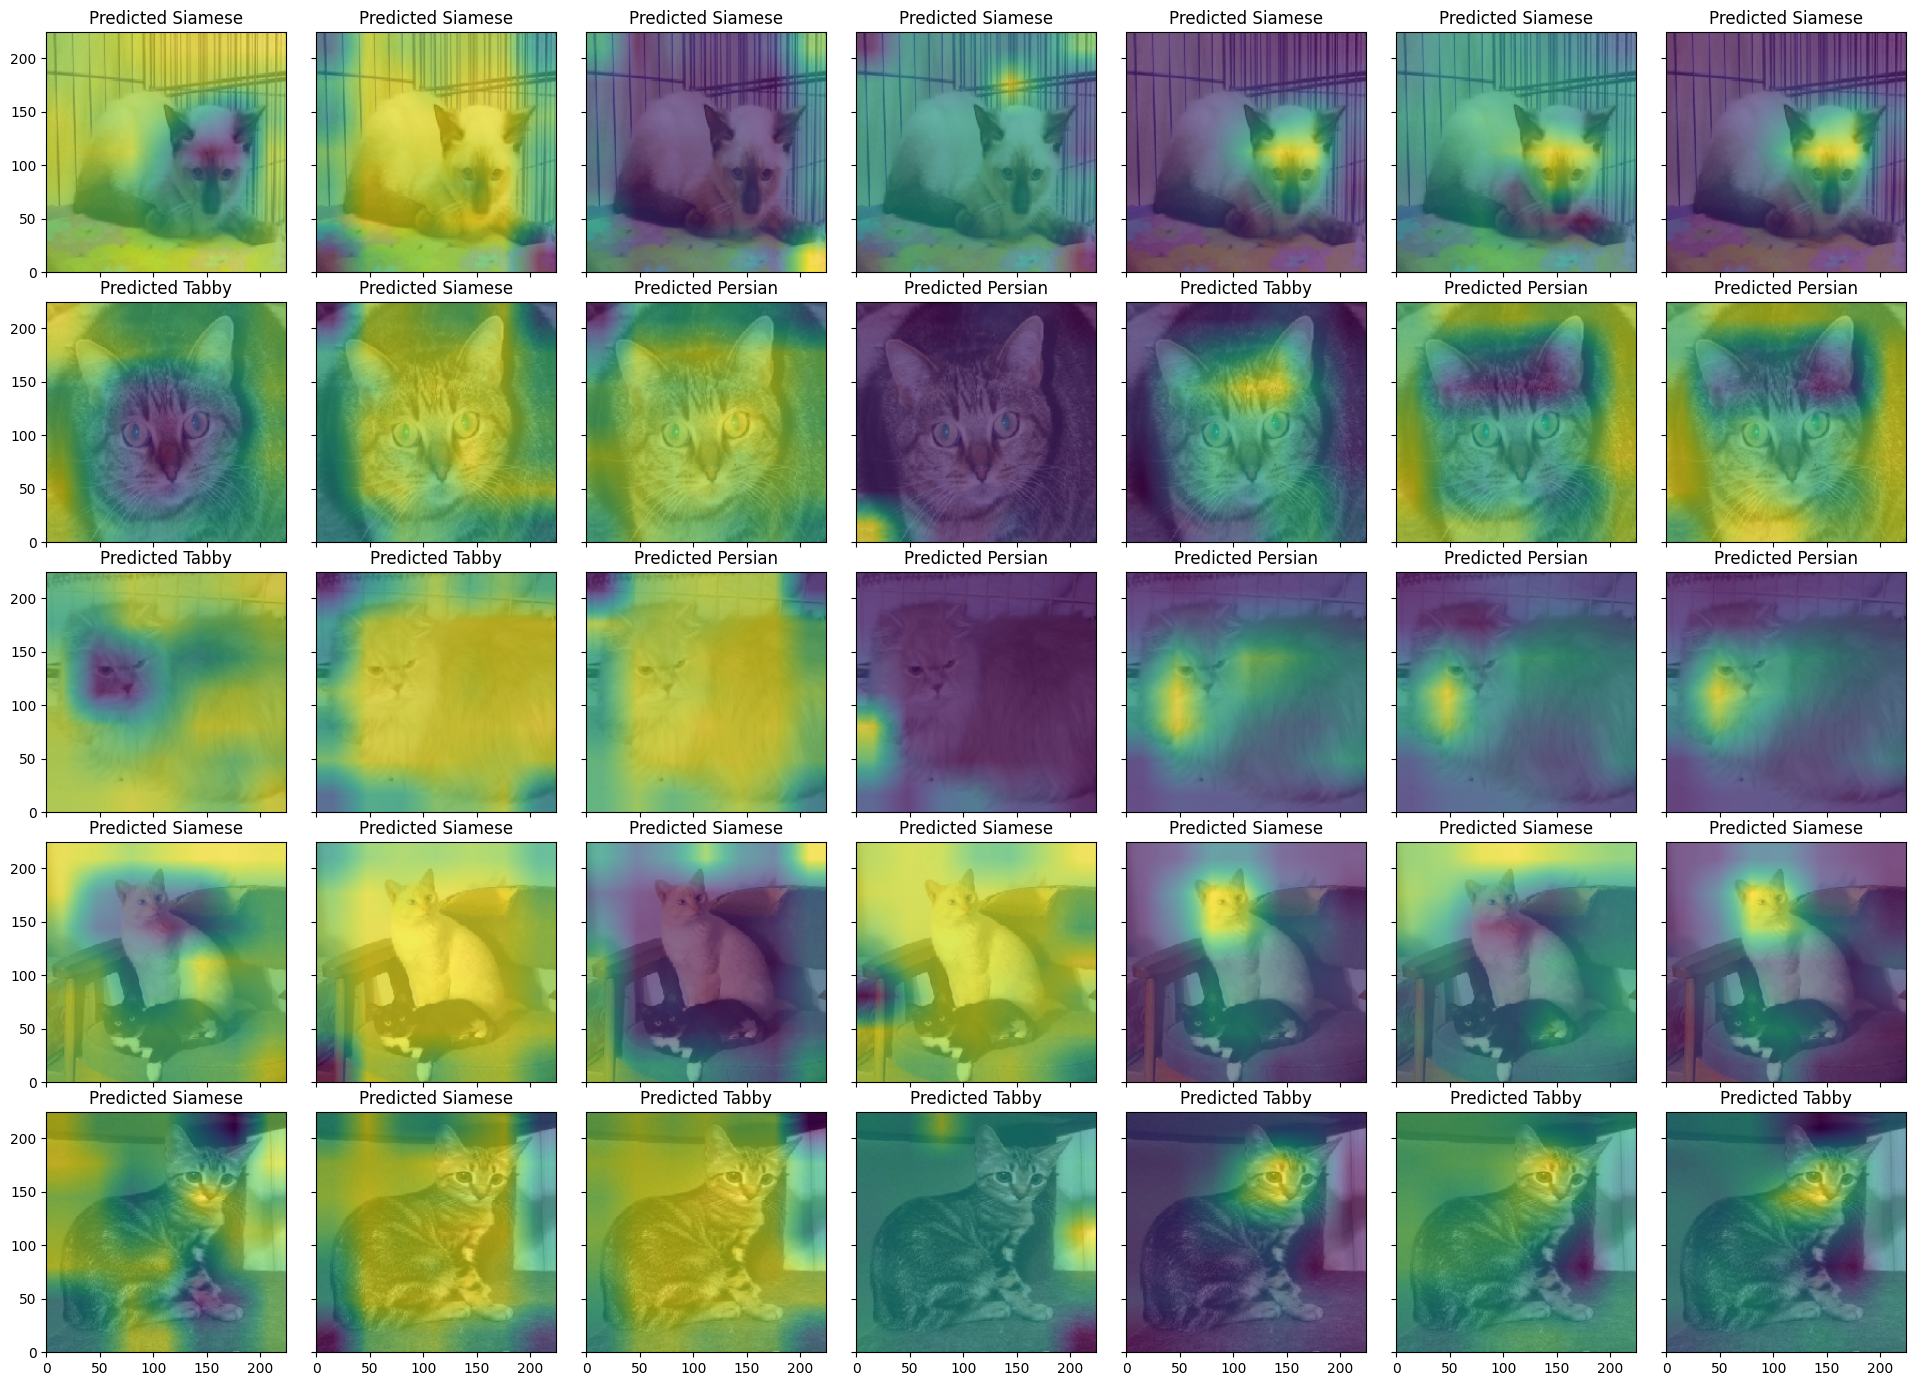
\includegraphics[height=2.5in]{imgs/cat_grids/2.png}
    \caption{2}
    \label{fig:2}
\end{figure}\begin{figure} [h]
    \centering
    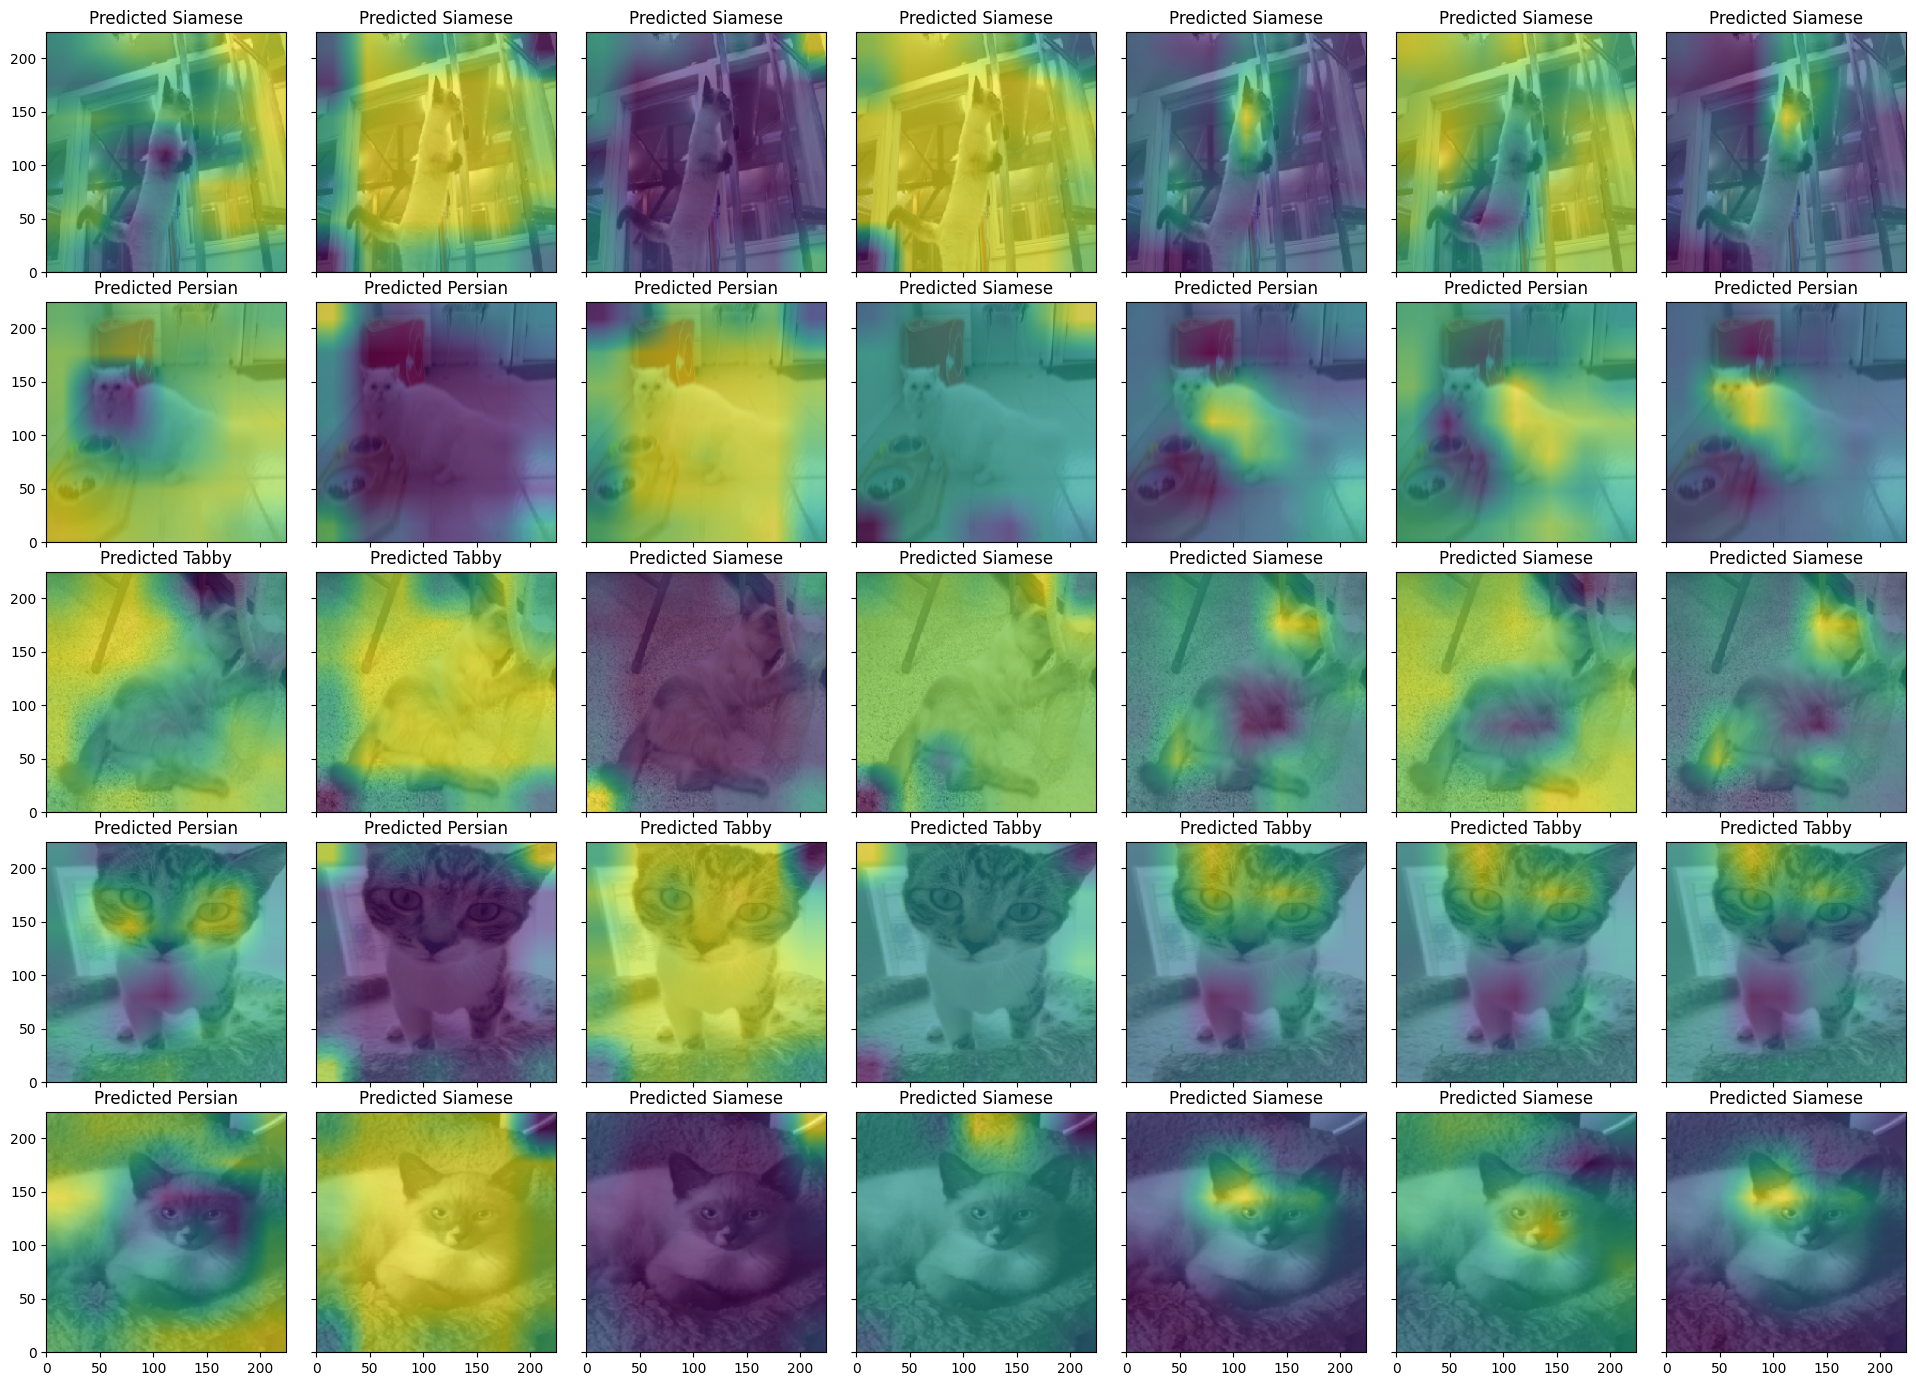
\includegraphics[height=2.5in]{imgs/cat_grids/3.png}
    \caption{3}
    \label{fig:3}
\end{figure}\begin{figure} [h]
    \centering
    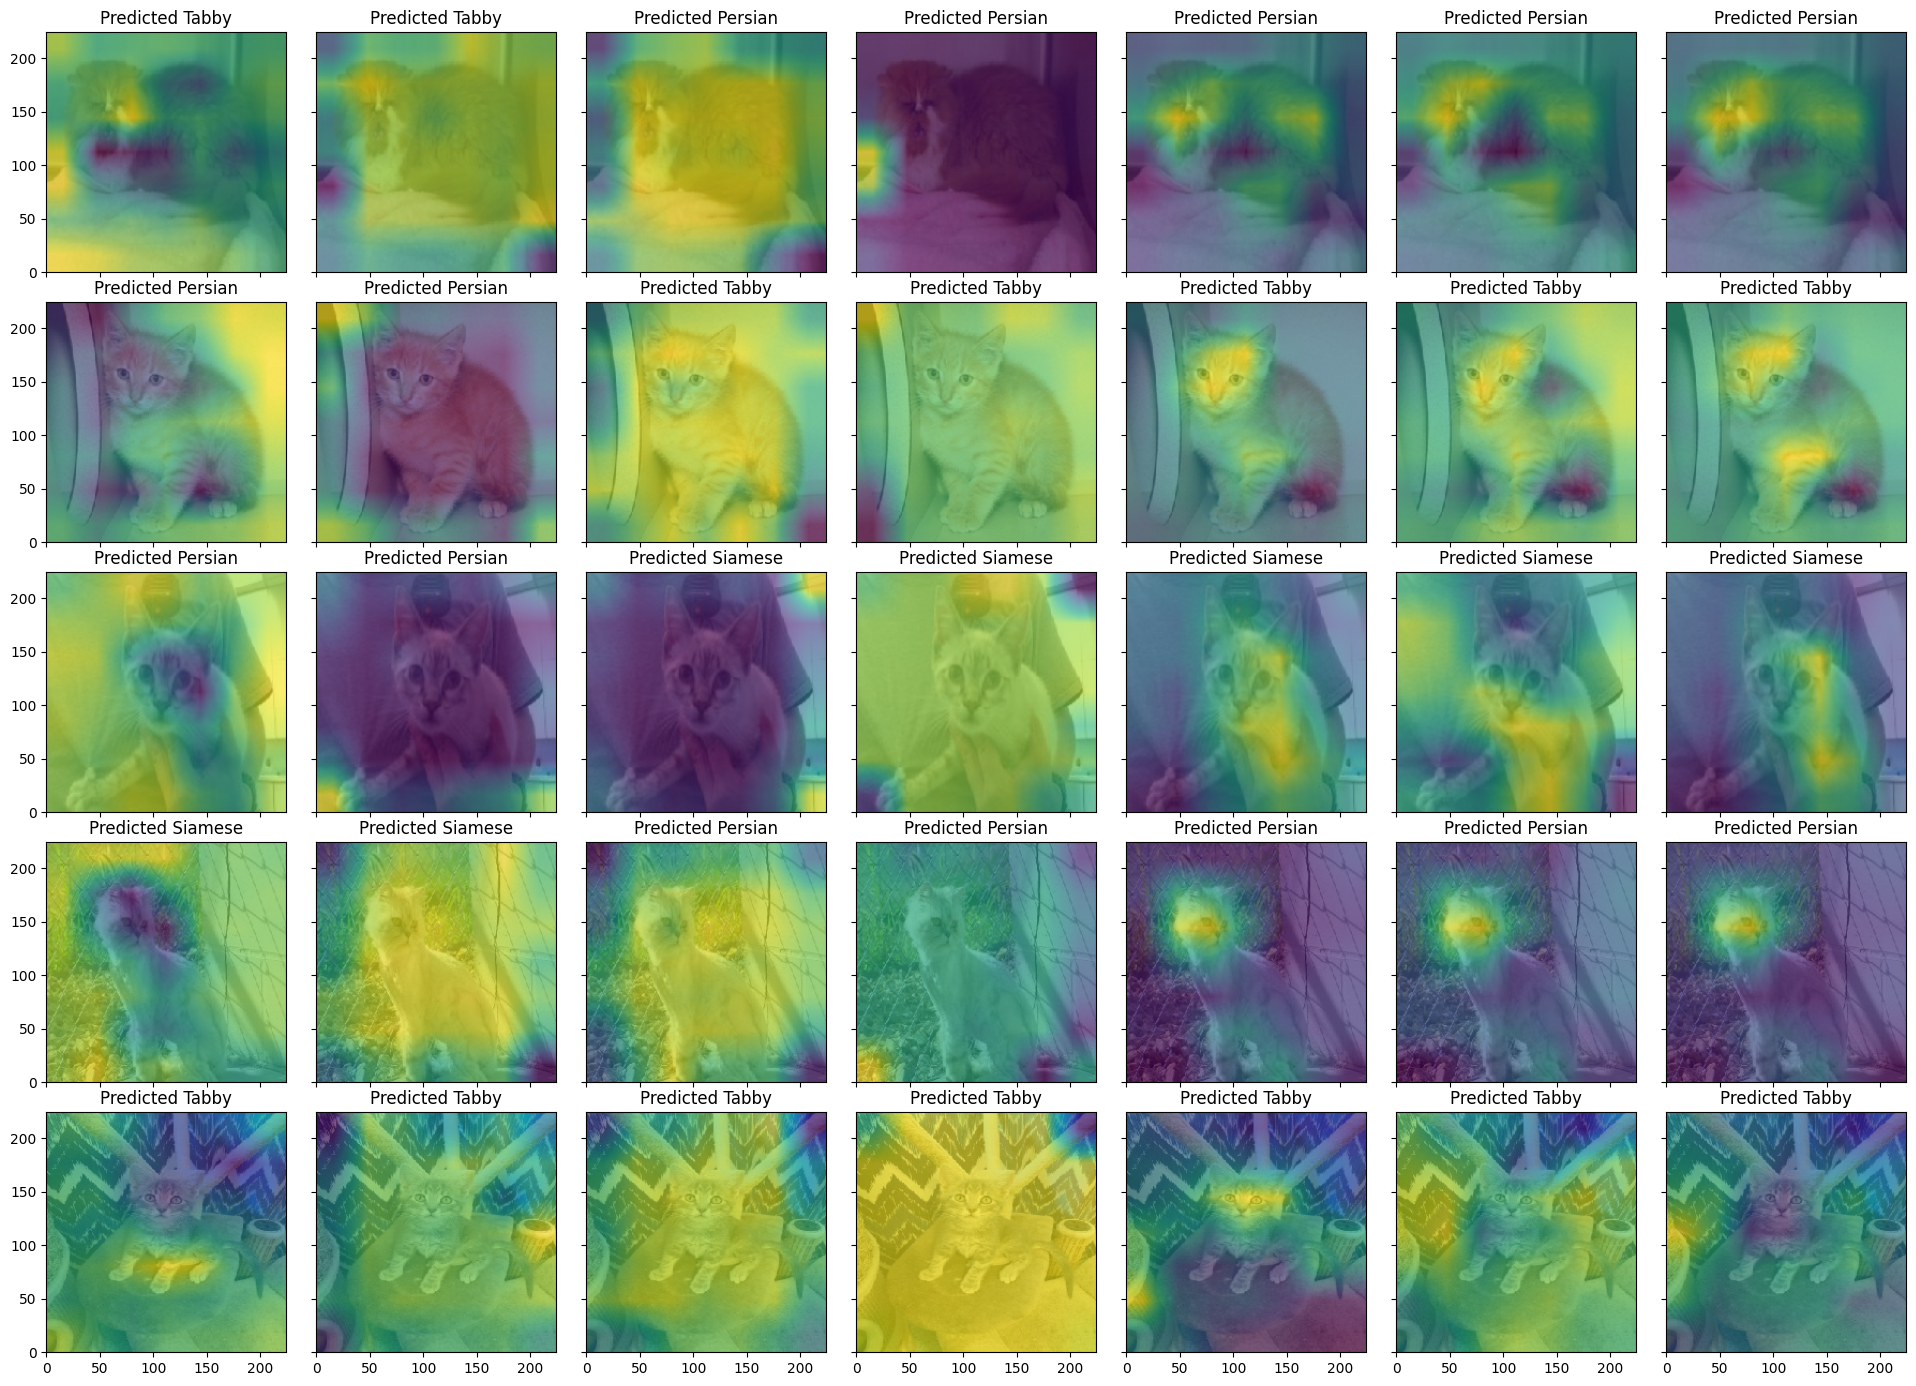
\includegraphics[height=2.5in]{imgs/cat_grids/4.png}
    \caption{4}
    \label{fig:4}
\end{figure}
\begin{figure} [h]
    \centering
    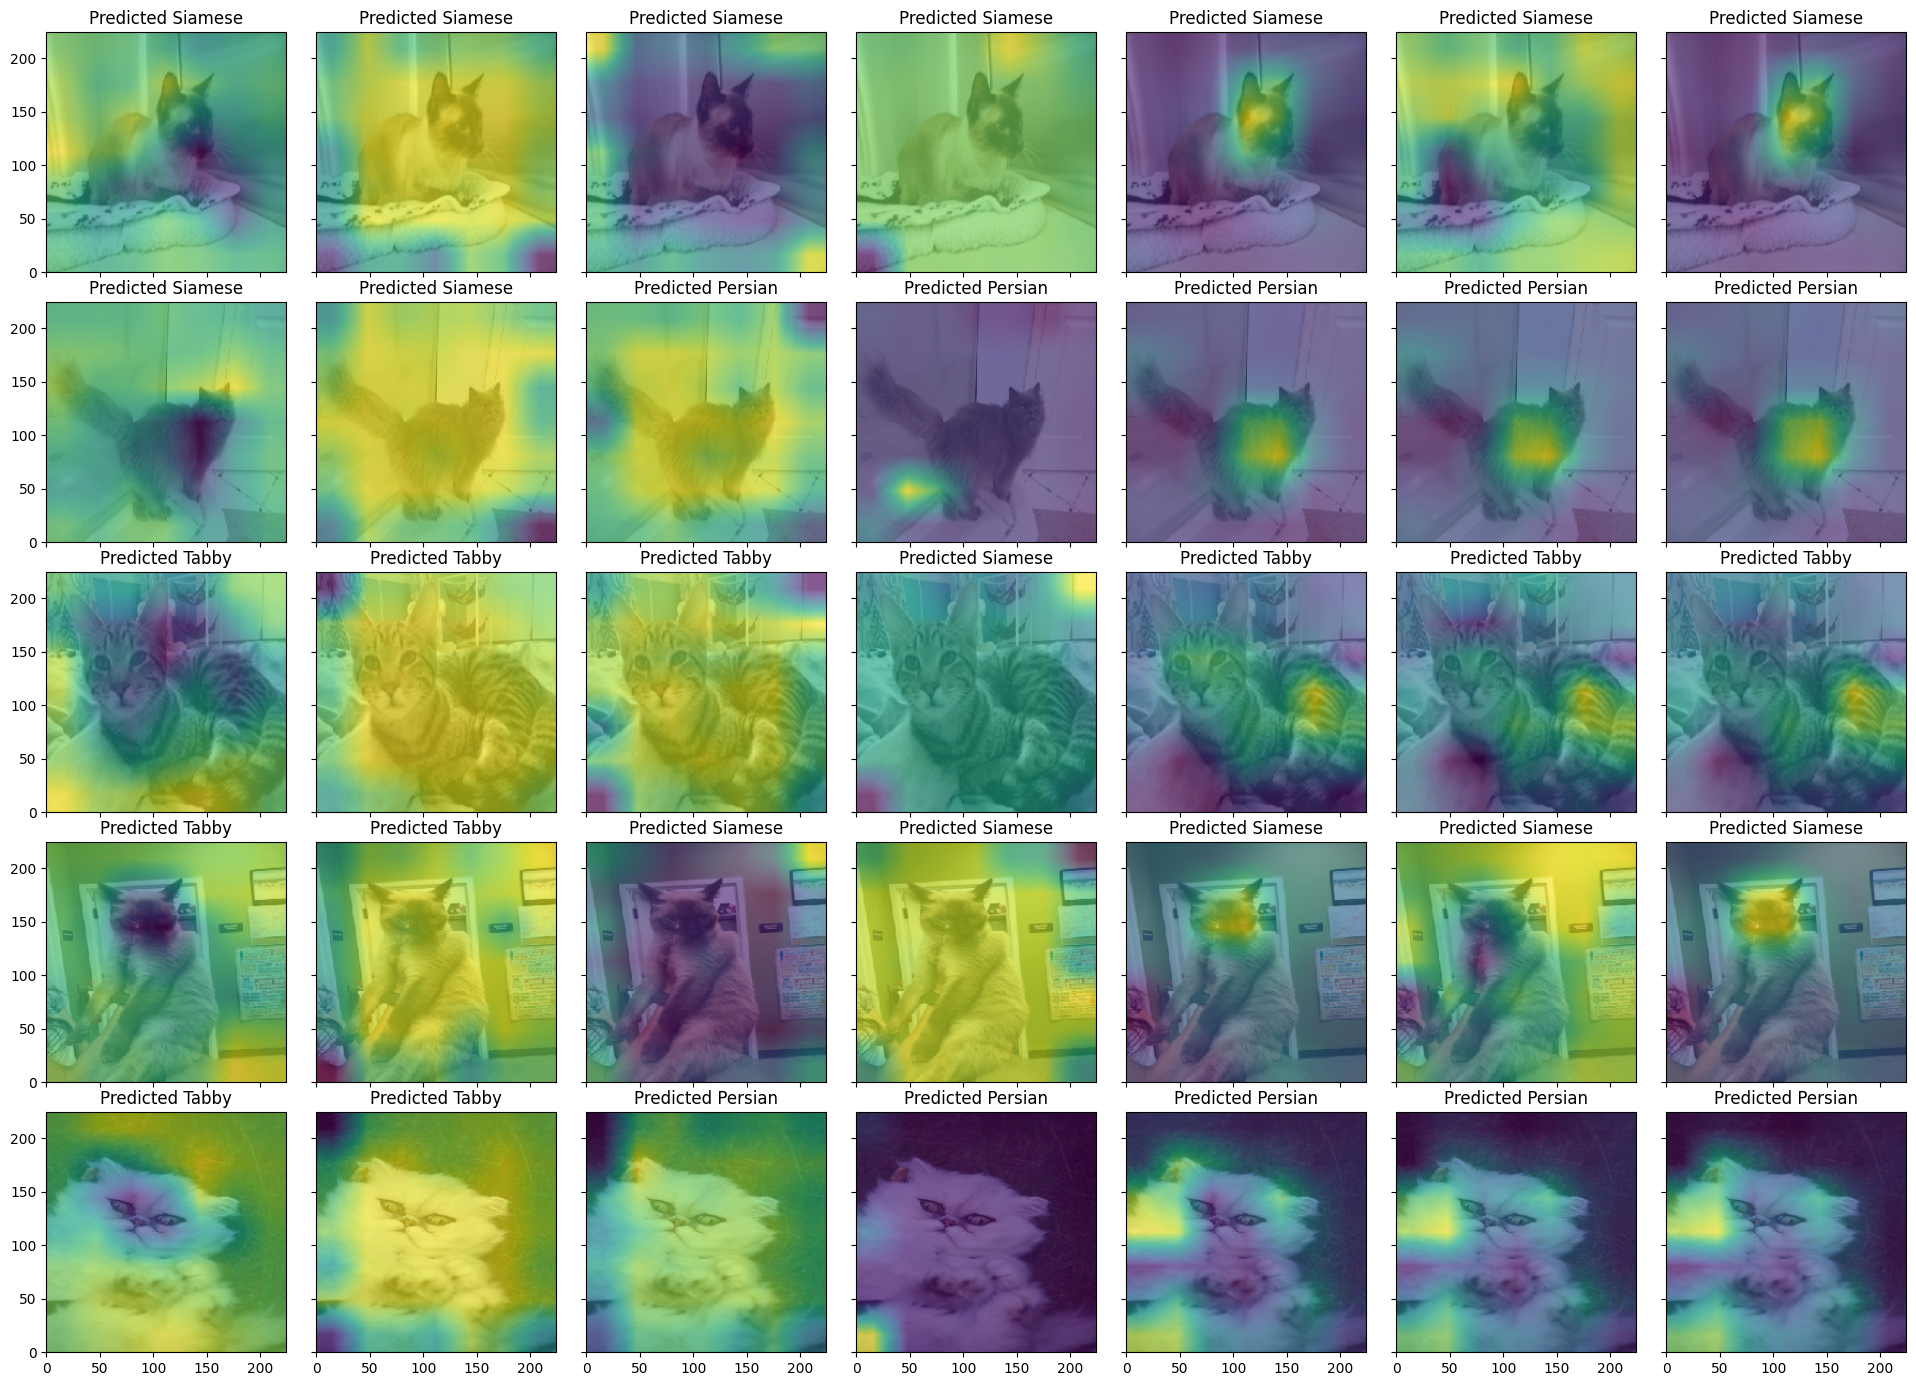
\includegraphics[height=2.5in]{imgs/cat_grids/5.png}
    \caption{5}
    \label{fig:5}
\end{figure}


\end{document}